\documentclass{article}

% if you need to pass options to natbib, use, e.g.:
% \PassOptionsToPackage{numbers, compress}{natbib}
% before loading nips_2016
%
% to avoid loading the natbib package, add option nonatbib:
% \usepackage[nonatbib]{nips_2016}

\usepackage[nonatbib, final]{nips_2017}

% to compile a camera-ready version, dd the [final] option, e.g.:
% \usepackage[final]{nips_2016}

\def\layersep{1.8cm}
\usepackage[utf8]{inputenc} % allow utf-8 input
\usepackage[T1]{fontenc}    % use 8-bit T1 fonts
\usepackage{booktabs}       % professional-quality tables
\usepackage{amsfonts}       % blackboard math symbols
\usepackage{nicefrac}       % compact symbols for 1/2, etc.
\usepackage{microtype}      % microtypography
\usepackage{mathtools}
\usepackage[compact]{titlesec}  
%%%%%%%%%%%%%%
% MATH
%%%%%%%%%%%%%%%
\usepackage{listings}
\usepackage{amsthm}
\usepackage{amssymb}
\usepackage{framed} 
\usepackage{amsmath}
\usepackage{amssymb}
\usepackage{relsize}
\usepackage{tikz}
\usepackage{xr}
% use Times
\usepackage{times}
% For figures
\usepackage{graphicx} % more modern
%\usepackage{epsfig} % less modern
\usepackage{subfigure} 
\usepackage{wrapfig}
% For citations
\usepackage[numbers]{natbib}

% For algorithms
\usepackage{algorithm}
\usepackage{algorithmic}
\usepackage{tikz-cd}


\newcommand{\BlackBox}{\rule{1.5ex}{1.5ex}}  % end of proof 

\newtheorem{theorem}{Theorem}
\newtheorem{example}[theorem]{Example}
\newtheorem{lemma}[theorem]{Lemma} 
\newtheorem{proposition}[theorem]{Proposition} 
\newtheorem{remark}[theorem]{Remark}
\newtheorem{corollary}[theorem]{Corollary}
\newtheorem{definition}[theorem]{Definition}
\newtheorem{conjecture}[theorem]{Conjecture}
\newtheorem{axiom}[theorem]{Axiom}

\numberwithin{theorem}{section}
\numberwithin{equation}{section}

\newcommand{\Sum}{\mathlarger{\mathlarger{\sum}}}

\newcommand{\rotB}{\scalebox{-1}[1]{B}}


\usetikzlibrary{backgrounds}
\usetikzlibrary{calc}
\usepackage{soul}
\usepackage{stackrel}

\usepackage{relsize}

\tikzset{fontscale/.style = {font=\relsize{#1}}
    }


\def\reals{{\mathbb R}}
\def\torus{{\mathbb T}}
\def\integers{{\mathbb Z}}
\def\rationals{{\mathbb Q}}
\def\naturals{{\mathbb N}}
\def\complex{{\mathbb C}\/}
\def\distance{\operatorname{distance}\,}
\def\support{\operatorname{support}\,}
\def\dist{\operatorname{dist}\,}
\def\Span{\operatorname{span}\,}
\def\degree{\operatorname{degree}\,}
\def\kernel{\operatorname{kernel}\,}
\def\dim{\operatorname{dim}\,}
\def\codim{\operatorname{codim}}
\def\trace{\operatorname{trace\,}}
\def\dimension{\operatorname{dimension}\,}
\def\codimension{\operatorname{codimension}\,}
\def\nullspace{\scriptk}
\def\kernel{\operatorname{Ker}}
\def\p{\partial}
\def\Re{\operatorname{Re\,} }
\def\Im{\operatorname{Im\,} }	
\def\ov{\overline}
\def\eps{\varepsilon}
\def\lt{L^2}
\def\curl{\operatorname{curl}}
\def\divergence{\operatorname{div}}
\newcommand{\norm}[1]{ \|  #1 \|}
\def\expect{\mathbb E}
\def\bull{$\bullet$\ }
\def\det{\operatorname{det}}
\def\Det{\operatorname{Det}}
\def\rank{\mathbf r}
\def\diameter{\operatorname{diameter}}

\def\t2{\tfrac12}

\newcommand{\abr}[1]{ \langle  #1 \rangle}

\def\newbull{\medskip\noindent $\bullet$\ }
\def\field{{\mathbb F}}
\def\cc{C_c}



% \renewcommand\forall{\ \forall\,}

% \newcommand{\Norm}[1]{ \left\|  #1 \right\| }
\newcommand{\Norm}[1]{ \Big\|  #1 \Big\| }
\newcommand{\set}[1]{ \left\{ #1 \right\} }
%\newcommand{\ifof}{\Leftrightarrow}
\def\one{{\mathbf 1}}
\newcommand{\modulo}[2]{[#1]_{#2}}

\def\bd{\operatorname{bd}\,}
\def\cl{\text{cl}}
\def\nobull{\noindent$\bullet$\ }

\def\scriptf{{\mathcal F}}
\def\scriptq{{\mathcal Q}}
\def\scriptg{{\mathcal G}}
\def\scriptm{{\mathcal M}}
\def\scriptb{{\mathcal B}}
\def\scriptc{{\mathcal C}}
\def\scriptt{{\mathcal T}}
\def\scripti{{\mathcal I}}
\def\scripte{{\mathcal E}}
\def\scriptv{{\mathcal V}}
\def\scriptw{{\mathcal W}}
\def\scriptu{{\mathcal U}}
\def\scriptS{{\mathcal S}}
\def\scripta{{\mathcal A}}
\def\scriptr{{\mathcal R}}
\def\scripto{{\mathcal O}}
\def\scripth{{\mathcal H}}
\def\scriptd{{\mathcal D}}
\def\scriptl{{\mathcal L}}
\def\scriptn{{\mathcal N}}
\def\scriptp{{\mathcal P}}
\def\scriptk{{\mathcal K}}
\def\scriptP{{\mathcal P}}
\def\scriptj{{\mathcal J}}
\def\scriptz{{\mathcal Z}}
\def\scripts{{\mathcal S}}
\def\scriptx{{\mathcal X}}
\def\scripty{{\mathcal Y}}
\def\frakv{{\mathfrak V}}
\def\frakG{{\mathfrak G}}
\def\aff{\operatorname{Aff}}
\def\frakB{{\mathfrak B}}
\def\frakC{{\mathfrak C}}

\def\symdif{\,\Delta\,}
\def\mustar{\mu^*}
\def\muplus{\mu^+}


\title{NN-body: Approximating Solutions to the $n$-body Problem using Neural Networks}

% The \author macro works with any number of authors. There are two
% commands used to separate the names and addresses of multiple
% authors: \And and \AND.
%
% Using \And between authors leaves it to LaTeX to determine where to
% break the lines. Using \AND forces a line break at that point. So,
% if LaTeX puts 3 of 4 authors names on the first line, and the last
% on the second line, try using \AND instead of \And before the third
% author name.

\author{
  William H.~Guss \\
  Unviersity of California, Berkeley\\
  Berkeley, CA 94720 \\
  \texttt{wguss@ml.berkeley.edu} 
}

\begin{document}
% \nipsfinalcopy is no longer used

\maketitle

\begin{abstract} 
The $n$-body problem, although simple in its formulation, is one of the most classic and unsolved problems in Newtonian mechanics. In this paper, we work towards a deeper understanding of the underlying dynamics of solutions by utilizing neural networks to approximate target states from initial conditions. Unlike previous numerical methods, neural networks are universal approximators which can capture and learn dynamics across variable timescales, without solving for intermediate solutions. We take advantage of one-shot prediction in order to analyze eigen-states \textbf{TODO: Finish abstract}
\end{abstract} 


\section{Background} Formally, the $n$-body problem considers the graviational dynamics of $n$ different point masses in $\mathbb{R}^3$. Let $m_i$, $p_i$, and $v_i$ denote the mass, position, and velocity of the $i$th point mass respectively. For every mass pair $i \neq j$, the force induced on mass $m_i$ by mass $m_j$ is given by Newton's law of gravitation
\begin{equation}\label{eq:forceindividual}
	F_{ij} = G m_i m_j \frac{p_j - p_i}{\left\|p_j - p_i\right\|^3}
\end{equation}
where $G$ is the graviational constant. Intuitively, $F_{ij}$ describes a force in the direction of $p_j$ (relative to $p_i$) whose magnitude is dependent on both the distance and combined mass potential of the two point-masses.

Integrating all force data from \eqref{eq:forceindividual} we yield that the acceleration applied to mass $m_i$ is
\begin{equation}
	\frac{d^2p_i}{dt^2}= G \sum_{\substack{k=1 \\ k\neq j}}^n  \frac{ m_j(p_j - p_i)}{\left\|p_j - p_i\right\|^3},
\end{equation}
where the acceleration is yielded by means of Newton's first law. In vector form,
\begin{equation}\label{eq:nbodyvec}
\begin{aligned}
	\frac{d^2p}{dt^2} &= G \left({\left\langle \left(p^{(i)} - p_i\right)\odot \frac{1}{\|p - p_i\|^3} \mathrel{}\middle|\mathrel{} m^{(i)} \right\rangle}\right)_{i=1}^n \\
	&= G  \tilde{M} \cdot \left(\left(p^{(i)} - p_i\right)\odot \frac{1}{\|p - p_i\|^3} \right)_{i=1}^n =: G \tilde{M}  \Pi(t)
\end{aligned}
\end{equation}
where $m^{(i)}, p^{(i)}$ are the full mass and position vectors with $i$th element removed, and $\tilde{M}$ is a matrix whose $i$th row is $m^{(i)}$.

In its full statement, the $n$-body problem can be stated as follows: given arbitrary initial position and velocity vectors, $p_0$ and $v_0$, does there exist an analytical solution $\scriptp$ to $\frac{d^2p}{dt^2} = G \tilde{M}  \Pi(t)$?


\begin{figure}
\begin{center}
	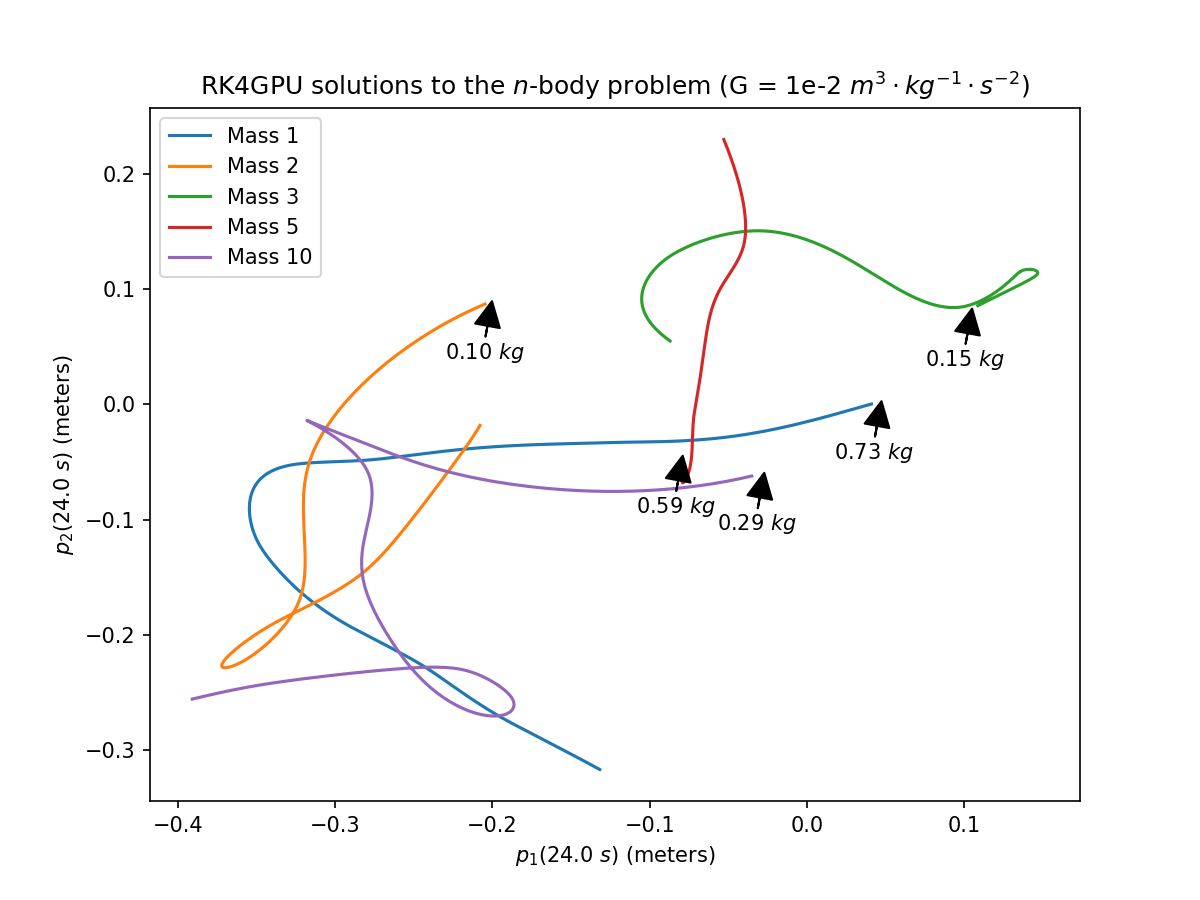
\includegraphics[width=0.49\textwidth]{solution.png} 
	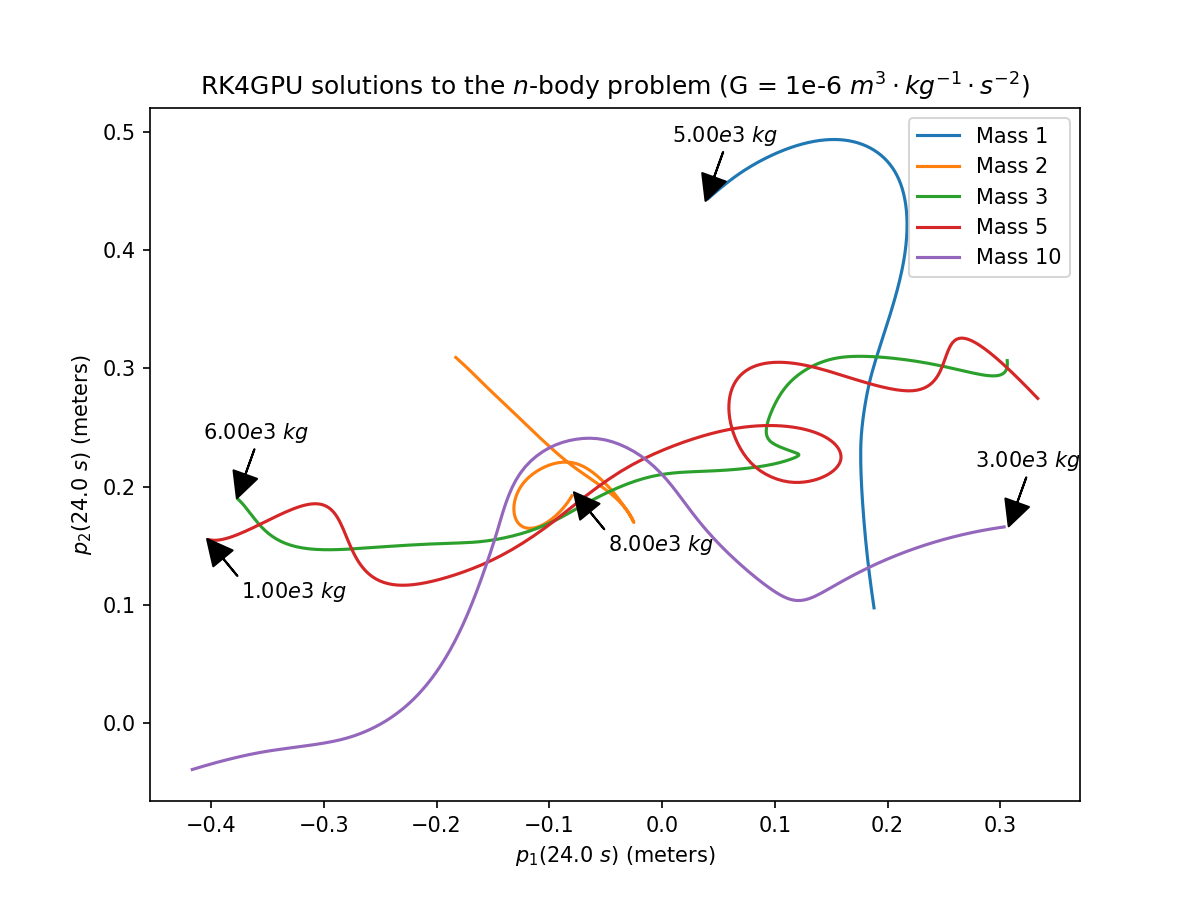
\includegraphics[width=0.49\textwidth]{solution2.png}
\caption{Seemingly chaotic solutions to the $n$-body problem with different iniital conditions and graivational constants as solved by RK4. Note the legends ommit some masses as activity localizes away from the origin with their initial conditions.}
\end{center}
\end{figure}

\section{Learning the $n$-body problem}
As of yet, there is no analytical solution to the arbitrary $n$-body problem, which given its simple formulation, raises questions as to our understanding of the complex dynamical patterns which emerge therefrom. Although numerical methods for solving \eqref{eq:nbodyvec} are sufficiently powerful for visualizing solutions, they are limited in their capacity for analysis; that is, on face value, such methods attempt to yield the temporally global solution by repeatedly and accurately modeling the local one. 

 In this paper, we approach numerical approximation from the alternative perspective of machine learning. Instead of iteratively arriving at a global solution, we will \emph{learn} the map $\pi: (p_0, v_0, t) \mapsto (p(t), v(t))$ using a family of \emph{hypothesis} function approximators whose analytical forms are condusive to statistical and spectral analysis globally in time.  Formally we will solve the following optimization problem, usually called a \emph{classification problem}.

 Let $\scriptd$ be the distribution induced by the jointly uniform random variables $P_0, V_0, T_0$. Given some hypothesis class $\scripth = \{h_\theta: \mathbb{R}^{3n} \times \mathbb{R}^{3n} \times \mathbb{R}
\times  [t_0, \infty)  \to  \mathbb{R}^{3n} \times \mathbb{R}^{3n} \}$ parameterized smoothly by $\theta \in \Theta,$ we wish to find $\theta^*$ such that
 \begin{equation}\label{eq:learning}
 	\theta^* = \arg\min_{\theta \in \Theta} \mathop{\mathbb{E}}_{(p_0, v_0, t) \sim \scriptd}\scriptl \Big( \pi(p_0,v_0,t), h_\theta(p_0, v_0, t)\Big),
 \end{equation}
 where $\scriptl$ is some monotonic function called a \emph{loss}. Usually we take $ \scriptl$ to be the $\ell_2$ norm.
 For intuition, note that if $h_{\theta^{*}} = \pi \in \scripth_\theta$ then the minimal expectation above is zero.

 In the foregoing regime, if we find a hypothesis class with which is sufficiently expressive, then the solution $h_{\theta_*}$ will approximate solutions to the $n$-body problem with arbitrary accuracy. It remains, however, to find such a hypothesis class $\scripth$ which also has the desired interpritability conditions and can yield novel statistical insights into the $n$-body problem. Luckily, artifical neural networks come close.

 \subsection{Deep Learning} \label{sec:dl}  Artificial neural networks (ANNs) are extremely powerful collection of machine learning algorithms, whose structure models the biological neuron closely. Over the past twenty years, the fields of computer vision and natrual language processing have seen exponential progress in solving machine perception as a result of deep learning. 

In its simplest form, deep learning considers the hypothesis class of all $\ell$-layer neural networks, $\scriptn_\ell$, such that
if $N: \mathbb{R}^n \to \mathbb{R}^m \in \scriptn_\ell$ then $N = N_\ell$ and the following recursion relation is defined for all $1 \leq j \leq \ell$,
\begin{equation}
	N_j(x) = \sigma\left(W_j N_{j -1}(x) + \beta_j\right);\;\;\;N_1(x) = x
\end{equation}
with matrices $W_\ell \in \mathbb{R}^{ n_{j} \times n_{j-1}},$ vectors $\beta_j \in \mathbb{R}^{n_j}$, and $n_1 = n, n_\ell = m.$ For the purposes of this work, it suffices to think of deep learning algorithms as functions which perform linear regression ($W, \beta$), apply some non-linearity ($\sigma$), and repeat this process $\ell$ times. 

The recent success of deep learning is in its name, the greater $\ell$ (the deeper the network), the more expressive power $\scriptn_\ell$ has. In the context of the $n$-body problem, $\scriptn_\ell$ is a \emph{universal approximator} for $\ell \geq 2$ and therefore is a proper candiate for the aforementioned hypothesis class. This means that given any continuous function $f: \mathbb{R}^n \to \mathbb{R}^m$ and any $\epsilon > 0$ there exists an $N \in \scriptn_\ell$ such that $\|N - f\|_\infty < \epsilon.$ 

Beyond expressivity, neural networks allow for inspection and interpretation of the mapping $f$ being learned via examination and analysis of the $\theta^* = (W, \beta)$ learned in \eqref{eq:learning}. In particular, one can analyze which states $x \in \mathbb{R}^n$ produce an output $y \in \mathbb{R}^m$ by updating some random initial $x_0$ so as to minimize $\|y - N(x)\|$. For the $n$-boduy problem, we therefore can determine eigenstates ($N(x) = \lambda x$) for the system and other such fixed points merely by applying this optimization method. Although there are many other such tools for inspecting the mappings learned in $\scriptn_\ell$, we shall restrict our attention to the foregoing.

\subsection{Training Neural Networks} Before we procede, we need specify if the optimization in $\eqref{eq:learning}$ is even possible when $\scripth = \scriptn_\ell$. Luckily, the observation that when $\sigma$ is twice--differentiable, as a function of $(W, \beta)$, $N(W,\beta; x)$ is twice-differentiable for all $x.$ As such, we then can seek local minima using \emph{gradient descent.} In the language of machine learning, the gradient descent algorithm changes the parameters $\theta$ such that $\scriptl$ decreases in the direction of greatest change; this direction of greatest decrease is the gradient $\nabla_\theta \scriptl.$ Therefore we define the \emph{gradient descent update rule} as follows,
\begin{equation}\label{eq:gradientdescent}
\begin{aligned}
	\theta_{t+1} = \theta_t - \lambda\frac{\partial L(\theta_t)}{\partial \theta} \\
\end{aligned}
\end{equation}
for some \emph{learning rate}, $\lambda \in \mathbb{R}.$ 

 In the context of neural networks, we need only compute $\partial \scriptl/\partial W$ and $\partial \scriptl/\partial \theta$ to move towards local optima. It's important to note that  there are no guarentees that \eqref{eq:gradientdescent} will converge to the global optima unless the function being optimized is \emph{g-convex} (geodesically convex). Despite this, the field of deep learning can attribute much if not all of its recent success to the empircal efficacy of \eqref{eq:gradientdescent} in training different neural networks, and therefore we shall assume convergence properties. 

 \subsection{NN-body Architecture}
To approximate solutions to \eqref{eq:nbodyvec}, we will choose a subset of $\scriptn_\ell$ over which to perform the optimization given in \eqref{eq:learning}. In deep learning, selection of different subsets of the foregoing hypothesis class, called architecutres, can have a significant impact on the accuracy of the models learned via gradient descent.


\textbf{TODO: Discuss architecture.}

 \section{Results}
With the learning problem defined, we now pose several questions as to approximation of the $n$-body problem via neural networks.

 First, is it possible to build some nueral network such that the loss on predictions of solutions far in the future is low and yet the computational complexity of the algorithm subsumes standard solvers in performance? In other words, is it possible to learn one-shot prediction of solutions $t$-timesteps in the future with subquadratic complexity? Second, using the methods described in section \ref{sec:dl}, what insights arise from analysis of eigenstates in these learned models, and how well do these eigenstates coorespond with true eigenstates of the $n$-body problem?

 \textbf{One-Shot Prediction.} In the first experiment, we train the NN-body architecture using gradient descent against data sampled from $\pi.$ We then measure performance by comparing the average loss of the neural network against the RK4 solutions to \eqref{eq:nbodyvec} on random initial conditions $(P_0, V_0, T_0),$ called a \emph{test set}, never shown to the neural network. Furthermore, we restrict the test set to particular timesteps and consider the performance degredation of the algorithm as $T_0 \to \infty.$ 

 Specifically, we train the neural network by drawing samples of $x_0 := (P_0, V_0, T_0)$ from a jointly uniformly random distribution. The samples are then solved by an RK4 solver applied to \eqref{eq:nbodyvec} implemented on a first GPU, and then the list of time-steps $\Gamma(x_0) = \{(P_\tau, V_\tau, h\tau)\}_{t=1}^{T_0/h}$, where $h$ is the stepsize for RK4, is then consolidated into initial-final pairs; that is, we let $B(x_0) := \{x_0\} \times \Gamma(x_0)$ where $\times$ is the cartesian product. The product $B(x_0)$ now consists of input and desired output pairs for which we will minimize $\scriptl(N(x), y)$ when $(x,y) \in B(x_0)$. We repeat this data generation and processing step untill the neural network $N$, trained on a second GPU, reaches sufficiently low error.

 \textbf{TODO: Discuss results.}


 \textbf{Eigenstate Analysis. }

\section{Conclusion}


% \input{sections/introduction}
% \input{sections/background}
% \input{sections/deep_funk_machines}
% \input{sections/topology}
% \input{sections/experiments}
% \input{sections/conclusion}

% \bibliographystyle{plainnatpllain}
% \bibliography{dfm}
% \newpage
% \input{sections/appendix}

\end{document}